\section{Automatic and Human Evaluation}
\label{sec:appendix:evaluation}


Up to this point, to evaluate our model, we have used standard automatic evaluation metrics for each particular task as reported in Table \ref{tbl:eval:metrics}. In this section, for the tasks of \st and \sst, we extend beyond these standard automatic metrics to include additional automatic and human evaluations to further assess our contributions. Automatic evaluations in this section reflect the robustness of our models in terms of noise and domains. Human assessment focuses on the preservation of speaker intention, as well as the subjective quality of the audio generated. To start, we introduce \blaser, a new, modality-agnostic evaluation metric that enables quality estimation for both speech and text.


\subsection{Modality-Agnostic Automatic Metric: \blaser} 
\label{sec:eval:blaser}

\paragraph{Description} \blaser is the new version of BLASER~\citep{chen-etal-2023-blaser}, which works with both speech and text modalities—hence being modality-agnostic. Like the first version, our approach leverages the similarity between input and output sentence embeddings. The new version uses SONAR embeddings (\ref{sec:appendix:data:sonar}), supports 83 languages in the speech modality and 200 in text, and is extendable to future encoders for new languages or modalities that share the same embedding space.
For the purposes of evaluating speech outputs (and unlike ASR-based metrics), BLASER offers the advantage of being text-free. 

More specifically, in \blaser, we take the source input, the translated output from any \sst, \st, or \mt model, and the reference speech segment or text, and convert them into SONAR embedding vectors ($h_\text{src}$, $h_\text{mt}$, and $h_\text{ref}$, respectively). For the supervised version of \blaser, these embeddings are combined and fed into a small, dense neural network that predicts an XSTS score for each translation output. For the unsupervised version, we use, similar to \cite{chen-etal-2023-blaser}, the average of source-translation and reference-translation cosine similarities.

In addition, we trained a reference-free version of the system called \blaser-QE (for Quality Estimation). \blaser-QE is a supervised model trained only with source and translation embeddings. It can be applied in settings where reference translations are missing or if their quality is questionable.


\paragraph{Data} The supervised version of \blaser was trained on the XSTS-annotated data (\cite{licht2022xsts}), which includes the same \sst annotations as in the original BLASER (\cite{chen-etal-2023-blaser}). Additional \sst, \st, and T2ST annotations come from a variety of other internal studies, including NLLB human evaluations \cite{nllb2022}, and 
\mt annotations are drawn from NLLB (\cite{nllb2022}). We filtered out all audio longer than 30 seconds because the SONAR encoders were not trained on long audio.

For the original BLASER data, train/test splits were reused. The other datasets were split randomly in 80/20 proportion so that the same source audio or text always goes to the same partition. Details on the data are reported in Table \ref{tab:blaser-data}.

\begin{table}[htb]
    \centering
    \small
    \begin{tabular}{lrrrrrrr}
\toprule
{\bf Data part} &  {\bf test size} &  {\bf train size} &  {\bf systems} &  {\bf langs} &   $\mathbf{\rho_{unsup.}}$&   $\mathbf{\rho_{sup.}}$ &  $\mathbf{\rho_{QE}}$ \\
\midrule
BLASER 1.0 \sst data    &       9804 &       10690 &       10 &      9 &                  0.51 &                0.56 & 0.53 \\
Other \sst data     &       5453 &       15904 &        8 &     13 &                  0.47 &                0.48  & 0.38\\
\st and T2ST data &       5205 &       10246 &        7 &      8 &                  0.49 &                0.54 & 0.51 \\

\mt data           &      20311 &       86776 &        2 &     59 &                  0.49 &                0.61 & 0.60\\
\midrule
{\bf All data}          &      40773 &      123616 &       24 &     62 &                  0.51 &                0.59 & 0.56 \\
\bottomrule
\end{tabular}
\caption{The data for \blaser: test and train size, number of systems and languages, Spearman correlation of unsupervised, supervised, and reference-free \blaser scores with XSTS labels on the test subset.}
\label{tab:blaser-data}
\end{table}


\paragraph{Training} 

For the supervised model, the architecture is the same as for the BLASER 1.0 model: a 3-layer perceptron with $tanh$ activations on top of 6 concatenated vectors of normalized embeddings and their derivatives: $[h_{ref};h_{mt};h_{src}\odot h_{mt};|h_{src}-h_{mt}|; h_{ref}\odot h_{mt};|h_{ref}-h_{mt}|]$. For the QE version, we used the same settings but with reference-free inputs: $[h_{src};h_{mt};h_{src}\odot h_{mt};|h_{src}-h_{mt}|]$.

We used the training code for BLASER 1.0 with a few modifications in the hyperparameters intended to mitigate overfitting: 50\% dropout, 0.1 weight decay, batch size of 1024, and full linear decay of the learning rate by the end of the training. To compensate for the increased batch size, we trained for 50 instead of 20 epochs.

\begin{table}[htb]
    \centering
    \small
\begin{tabular}{lrrrrrrr}
\toprule
& \multicolumn{6}{c}{\bf $\uparrow$Pearson Correlation}\\\cmidrule{2-7}
{\bf Model} &  eng-deu &  eng-spa &  eng-fra &  spa-eng &  fra-eng &  rus-eng &  {\bf average} \\ 
\midrule
BLASER 1.0 unsup & 0.32 & 0.58 & 0.64 & 0.50 & 0.48 & 0.43 & 0.49 \\
\blaser unsup & \textbf{0.37} & 0.75 & 0.71 & 0.59 & 0.57 & 0.49 & 0.58 \\
\blaser QE    & 0.34 & 0.73 & 0.71 & 0.54 & 0.48 & 0.45 & 0.54 \\
BLASER 1.0 sup   & 0.33 & 0.75 & 0.71 & 0.58 & \textbf{0.57} & \textbf{0.53} & 0.58 \\
\blaser sup   & 0.36 & \textbf{0.75} & \textbf{0.73} & \textbf{0.58} & 0.56 & 0.50 & \textbf{0.58} \\
\bottomrule
\end{tabular}
\caption{Pearson correlations of unsupervised and supervised BLASER models with XSTS scores on the BLASER 1.0 test data.}
\label{tab:blaser-corrs}
\end{table}

\paragraph{Results} Table \ref{tab:blaser-corrs} presents the performance of unsupervised and supervised BLASER on the BLASER 1.0 test data. The unsupervised 2.0 model slightly outperforms its predecessor. The supervised v1.0 and v2.0 models have the same average correlation with human judgments. Because \blaser supports more languages, we used this for evaluations.
 
The last three columns in Table \ref{tab:blaser-data} present correlations of the 2.0 model's predictions with XSTS scores for all data partitions. Based on the results, the supervised model outperforms the unsupervised on each partition. The reference-free model scores between them in most cases, but for the new \sst data, its performance is below that of the unsupervised model. We hypothesized that on this subset, references sometimes diverge from the sources, either due to errors of speech segmentation or synthesis, or due to non-literal translation that makes sense only in the context. A manual examination of a few samples corroborates this hypothesis, but more analysis of the role of reference in BLASER models is required in the future.
Full \blaser scores for \mfourt models are reported in table \ref{tbl:modeling:spbleu}. Additionally, the next section \ref{subsec:appendix:humanmetrics} reports the corresponding correlations of \blaser scores with human scores.






\subsection{Human Evaluation}
\label{subsec:appendix:humanmetrics}


Human evaluation is a vital tool in assessing the quality of our systems. We first briefly describe related work in the area, followed by a detailed description of the entire human evaluation process, including protocols, data, and calibration. 

\paragraph{Related work.} Human evaluation has been widely applied to machine translation in the scientific community. Two of the most popular models of human evaluation are deployed within the context of International Evaluation Campaigns. The WMT conference \citep{kocmi-EtAl:2022:WMT} asks participants to evaluate the outputs of translation systems using a pre-defined protocol, typically that of Direct Assessment \citep{grahametal2013directassessment}.  
Beyond this text-based evaluation, the IWSLT Evaluation Campaign covers speech translation. As an example, the speech-to-speech track\footnote{https://iwslt.org/2023/s2s} evaluates speech output quality in four dimensions. The first one is translation quality, which focuses on capturing meaning, and annotators rank target audio between 1 and 5. The rest of the dimensions cover naturalness, including voice and pronunciation, clarity of speech for comprehension, and sound quality, which takes into account noise and other artifacts. These criteria are used as an alternative to the Mean Opinion Score (MOS).


\subsubsection{Human Evaluation Protocols} 

Similar to the related work aforementioned, for \st evaluation, we used the XSTS protocol to assess translation quality. For the \sst task, we evaluate using two protocols: XSTS for translation quality, and MOS to assess naturalness. 

\paragraph{XSTS.}  XSTS \citep{licht2022xsts} evaluates translation quality in terms of semantic meaning preservation, and has previously been used to evaluate the NLLB models \citep{nllb2022}.  While XSTS was originally designed to evaluate text, the protocol is effectively modality agnostic, and we required only small adaptations in order to support \sst and \st tasks.   For instance, the \sst and \st versions of the protocol required additional instructions for annotators regarding the treatment of non-speech tags (e.g. \texttt{<laugh>}), which the annotators were instructed to ignore, and how they should consider pauses and non-speech noises (they are instructed to ignore these as well).

On the execution logistics side, conversations with vendors used for our evaluation work indicated that the evaluation of \sst translations seemed to require a higher cognitive load for the annotators than \mt (as a result of not being able to experience the source and target simultaneously), and thus was slower to conduct. 



\paragraph{XSTS annotation and calibration process.} During annotation, 3 annotators examined each source-target audio pair (or audio-text pair) and evaluated the item for semantic similarity using the XSTS protocol. Prior to annotating, all annotators went through a set of monolingual English `practice' evaluations with score justifications.  To expedite evaluation, more than 3 (up to 30 in our case) annotators were used per language pair; each evaluated sentence pair was shown to 3 annotators, assigned essentially randomly, and with calibration set items intermixed in the evaluation. In cases where the 3 annotators had a disagreement of score values of 2 or more, 2 additional annotators evaluated the same item again, bringing the total to 5 evaluator scores for those items. The median score over annotators of the same audio pair was then taken for each evaluation sentence pair; the median is used for robustness.  The process was the same for both \sst and \st evaluations. For overall direction scores, we report the mean of this median score (or some aggregate, such as the fraction of sentences with a median XSTS score above a given threshold) across all evaluated items in the dataset generated by a particular system in a language direction. Calibration set items received the exact same treatment, resulting in 1 score per sentence pair per annotator pool, and language-level scores were calibrated using the mean score on the calibration set for the crew of annotators evaluating a given language direction; the calibration set and methodology is described below.

To enable interlanguage comparison of model quality, a mono-lingual "cross-lingual calibration set" \citep{licht2022xsts} was generated and included in the evaluation, and scores were calibrated using the `moderated calibration' methodology established previously \citep{licht2022xsts,nllb2022}.  The calibration process was found to reduce language-level annotator biases and has been shown to improve correlation with automatic metrics as a result. %
Running a calibration set or `gold set' of items with a known score, even one much-reduced in size (e.g., 50–100 items instead of the 500 here) is useful as a diagnostic tool for ensuring annotation quality, even if one is not intending on doing interlanguage calibration.  Annotator crews sufficiently `out of calibration' can be identified, and their results excluded, or additional training can be conducted to improve their performance.  

\paragraph{MOS.} To evaluate and compare generated speech quality for the \sst task, we used a standard Mean Opinion Score (MOS) protocol to evaluate naturalness, quality of sound, and clarity of speech of our generated audio. MOS methodology has been in use in the telecommunications industry for decades and it was standardized in Recommendation ITU-T P.800. 
In particular, the adapted guidelines that we used for the MOS evaluation include the following instructions:
\begin{enumerate}
\item \textbf{How clear is the speech? }
Recordings with clear speech and no mumbling and unclear phrases should be given a high score. Recordings with a large amount of mumbling and unclear phrases should be given a low score.
\item \textbf{How good is the sound quality?}
Recordings with clean audio and no noise and static in the background should be given a high score. Recordings with a large amount of noise and static in the background should be given a low score.
\item \textbf{How natural is the speech?}
Recordings that sound human-like, with natural-sounding pauses, stress, and intonation, should be given a high score. Recordings that sound robotic, flat, or otherwise unnatural should be given a low score. 
\end{enumerate}

For each of these questions, annotators are instructed to provide a Likert score (1-5). The MOS evaluations were conducted on the same generations as those evaluated with the XSTS protocol, with the exclusion of the cross-lingual calibration set items, and we elected to only evaluate a more limited sample of language directions into English (as MOS characteristics were not expected to be strongly dependent on the input language). Similar to XSTS, 3 annotators scored each generation for most languages evaluated, with some languages (\texttt{cat}, \texttt{fin}, \texttt{hin}, \texttt{ind}, \texttt{ita}, \texttt{kor}, \texttt{por}, \texttt{ron}, \texttt{swh}, \texttt{tel}, \texttt{tha}, \texttt{tur}, \texttt{urd}, \texttt{vie}) only receiving scores from a single annotator per item (this balanced the need for language coverage with budgetary constraints). The median of annotator scores is collected for each item, and aggregate scores are presented in the paper. Unlike XSTS, additional annotators were not consulted when scores disagreed and calibration was not performed.


\subsubsection{Evaluation Framework}

\paragraph{Dataset} Human evaluations were conducted utilizing the `test' partition of the \fleurs dataset \citep{fleurs2022arxiv}.  The \fleurs `test' partition provides up to 350 sentences sourced from the FLORES-101 dataset \citep{flores101:2021} for each supported language (\fleurs supports 102 languages). Each sentence has up to 3 recorded audios spoken by different speakers (depending on which recordings passed quality review), along with the associated FLORES-101 text. The quality review requirement means that each language may not have a recording for all 350 sentences and that for those sentences that do have recordings, not all three speaker recordings may be present.

When conducting an evaluation of a translation system for a particular language direction, we filtered down the \fleurs data to a subset of sentences that have recordings in both languages in order to have a common, bidirectional evaluation set per-language pair. We do this to ensure \st and \sst evaluations both use an identical set of sentences. Because the coverage of \fleurs varies per language, the subset of items present in the evaluation set varies per language and thus also per language pair; though there is a majority of items common across languages, and we believe the scores to be largely comparable as they were drawn from the same domain.  

When preparing \fleurs to be used as a human reference set, pairings had to be made between distinct readers in the source language and readers of the equivalent \fleurs item in the target language.  When possible, these pairings were made to match user gender (53\% of the time over the entirety of the \fleurs test partition, varying significantly between languages paired with English), and mixed-gender matches had to be made for the remaining 47\% of items. We elected to limit human evaluation to 2 unique readings per \fleurs sentence at most.  %

 


\newcommand{\evallangs}{{24}}
\begin{table}
\centering

\small
\begin{threeparttable}
\begin{tabular}{llllp{3cm}}
\toprule
{\bf Modality} & {\bf Protocol} & {\bf Direction} & {\bf Systems} & {\bf Languages} \\
\midrule
\st & XSTS & \xeng & 
\makecell[l]{\whisperlarge\\\mfourtlg$^*$\tnote{1}} &
\evallangs\tnote{2}
\\ 
\st & XSTS & \engx & \mfourtlg$^*$ &
\evallangs
\\
\midrule
\sst & XSTS &\xeng &
\makecell[l]{\whisperlarge+\yourtts\\\mfourtlg} & 
\evallangs
\\
\sst & XSTS & \engx  & \mfourtlg &
\evallangs
\\
\midrule 

\sst & MOS  & \xeng & 
\makecell[l]{\whisperlarge+\yourtts\\\mfourtlg} & 
8 (arb, cmn, fra, hin, rus, spa, tel, tur) \\
\sst & MOS  & \engx & \mfourtlg &
\evallangs
\\
\bottomrule
\end{tabular}
\begin{tablenotes}
\item[1] \mfourtlg$^*$ refers to the \mfourtlg model using \texttt{fairseq} for generations instead of \fairseq, but \st performance was on average within 0.5 \bleu between the two.
\item[2] Bengali, Catalan, Dutch, Finnish, French, German, Hindi, Indonesian, Italian, Japanese, Korean, Mandarin Chinese, Modern Standard Arabic, Portuguese, Romanian, Russian, Spanish, Swahili, Tagalog, Telugu, Thai, Turkish, Urdu, and Vietnamese.
\end{tablenotes}
\end{threeparttable}
\caption{\label{table:evalsummary} Summary of evaluations: languages, modalities, models, and protocols used in human evaluations. Modalities and protocols in parentheses are not presented in this paper but will be shared in a later update.}
\end{table}



\paragraph{Language directions, modalities, and systems evaluated} We list the languages and modalities evaluated with each protocol in Table \ref{table:evalsummary}. Language selections were made by balancing a mix of resource availability for human annotations. The final language sample captures a large human population while also representing a mix of high and mid-resource languages.

For the \st and \sst tasks, we have XSTS evaluations of \evallangs{} languages in the \xeng direction for both the \mfourtlg and \whisperlarge models, where generations from the \mfourtlg model were made using a slightly earlier version via \texttt{fairseq} (instead of \fairseq) but \st performance has less than 0.5 \bleu average difference. For \engx, we have evaluations for the same languages but only for the \mfourtlg model (with \texttt{fairseq} generations). Additionally, we have evaluations for a human reference system (i.e. the \fleurs data itself) for all languages in each direction.

We only evaluated direct models for \st and plan to extend the benchmarking to 2-stage cascaded systems in future work for \engx. For \sst, we do not evaluate \engx benchmarks due to the complexity involved in running monolingual TTS models for all the target directions. However, in the future, we plan to build such baselines using systems like MMS-TTS \cite{mms}; we have experimented using these same systems in other sections of this paper, e.g. for the purpose of extending text-based responsible AI datasets to speech (Section \ref{subsec:biasexperimental}). 

For the \sst task, we used the MOS protocol to evaluate for all \evallangs{} in the \engx direction. Since we do not expect MOS scores to be strongly sensitive to input language when evaluating English output speech, we evaluated a smaller language set in the \xeng direction (only 8 languages).




\subsubsection{Human Evaluation Results}


\paragraph{XSTS results for the \st task} %

\begin{table}
\begin{tabular}{rrccc}
\toprule
{\bf Direction} & {\bf System} & {\bf Avg. XSTS (\st)} & {\bf \% 3+} & {\bf \% 4+} \\
\midrule
\engx & Human reference & 4.69 & 95.98 & 78.66 \\
 & \mfourtlg & 4.53 & 87.69 & 73.28 \\
\midrule
& Human reference & 4.67 & 95.23 & 76.86 \\
\xeng & \whisperlarge & 4.05 & 70.11 & 58.00 \\
& \mfourtlg & {\bf 4.16} & {\bf 72.51} & {\bf 59.86} \\
\bottomrule
\end{tabular}
\caption{For \st task: overall average XSTS human evaluation results into and out of English, over all \evallangs{} evaluated languages.  Results were computed for each language direction (see Table \ref{table:fullXSTSresultsst} for full language-level results).  \%3+ and  \%4+ refer to the percent of a language's evaluated sentences with median scores equal to or greater than 3 and 4 respectively.}
\label{tab:XSTShighlevelsummaryst}
\end{table}


\begin{table}
\centering
\begin{threeparttable}
\scriptsize
\begin{tabular}{ll|ccc|ccc|ccc|c}
\toprule
\textbf{Direction} & \textbf{Lang} & \multicolumn{3}{c}{\textbf{XSTS (calibrated)}} & \multicolumn{3}{c}{\textbf{\% XSTS 3+}} & \multicolumn{3}{c}{\textbf{\% XSTS 4+}} & \textbf{Items} \\
 &  & Seamls\tnote{1} & Wspr\tnote{2} & Hum\tnote{3} & Seamls & Wspr & Hum & Seamls & Wspr & Hum &  \\
\midrule
\engx & arb & 4.53 & -- & 4.61 & 90.2 & -- & 96.8 & 71.7 & -- & 72.9 & 410 \\
 & ben & 4.35 & -- & 4.49 & 92.1 & -- & 96.8 & 64.2 & -- & 73.0 & 629 \\
 & cat & 4.73 & -- & 4.82 & 90.1 & -- & 95.9 & 82.6 & -- & 85.0 & 638 \\
 & cmn & 4.03 & -- & 4.69 & 70.1 & -- & 98.0 & 41.7 & -- & 69.7 & 636 \\
 & deu & 4.61 & -- & 4.75 & 88.4 & -- & 96.1 & 72.4 & -- & 77.5 & 612 \\
 & fin & 4.37 & -- & 4.66 & 75.5 & -- & 93.0 & 52.1 & -- & 61.2 & 632 \\
 & fra & 4.76 & -- & 4.83 & 92.0 & -- & 98.5 & 83.3 & -- & 83.3 & 538 \\
 & hin & 4.55 & -- & 4.51 & 98.2 & -- & 97.4 & 77.6 & -- & 74.5 & 388 \\
 & ind & 4.81 & -- & 4.84 & 97.6 & -- & 98.5 & 83.8 & -- & 85.8 & 544 \\
 & ita & 4.59 & -- & 4.56 & 97.1 & -- & 97.4 & 93.8 & -- & 90.2 & 612 \\
 & jpn & 4.09 & -- & 4.74 & 66.7 & -- & 92.6 & 53.9 & -- & 79.8 & 514 \\
 & kor & 4.58 & -- & 4.76 & 85.7 & -- & 94.7 & 66.3 & -- & 76.7 & 356 \\
 & nld & 4.72 & -- & 4.67 & 88.4 & -- & 94.0 & 78.2 & -- & 62.7 & 335 \\
 & por & 4.79 & -- & 4.8 & 95.7 & -- & 97.6 & 92.2 & -- & 90.8 & 632 \\
 & ron & 4.71 & -- & 4.88 & 89.3 & -- & 98.4 & 77.9 & -- & 86.8 & 619 \\
 & rus & 4.56 & -- & 4.76 & 82.9 & -- & 94.3 & 73.2 & -- & 78.7 & 597 \\
 & spa & 4.69 & -- & 4.59 & 89.1 & -- & 96.5 & 82.0 & -- & 62.9 & 623 \\
 & swh & 4.52 & -- & 4.81 & 82.0 & -- & 93.1 & 76.6 & -- & 90.8 & 466 \\
 & tel & 4.5 & -- & 4.49 & 96.6 & -- & 97.3 & 89.8 & -- & 88.0 & 442 \\
 & tha & 4.18 & -- & 4.65 & 78.2 & -- & 94.7 & 46.5 & -- & 70.0 & 643 \\
 & tur & 4.61 & -- & 4.84 & 88.7 & -- & 97.9 & 74.7 & -- & 87.5 & 566 \\
 & urd & 4.39 & -- & 4.52 & 91.2 & -- & 95.1 & 68.9 & -- & 76.0 & 283 \\
 & vie & 4.63 & -- & 4.65 & 93.0 & -- & 95.6 & 85.1 & -- & 84.6 & 611 \\
 \midrule
\xeng & arb & 4.29 & 3.82 & 4.59 & 81.7 & 62.7 & 95.1 & 62.7 & 43.4 & 72.7 & 410 \\
 & ben & 4.03 & 2.84 & 4.51 & 78.1 & 37.0 & 97.6 & 51.8 & 16.2 & 74.7 & 629 \\
 & cat & 4.72 & 4.59 & 4.79 & 89.3 & 84.2 & 95.3 & 81.8 & 76.8 & 82.0 & 638 \\
 & cmn & 3.75 & 4.04 & 4.55 & 58.5 & 67.8 & 94.0 & 37.1 & 48.1 & 59.7 & 636 \\
 & deu & 4.64 & 4.69 & 4.81 & 88.4 & 90.2 & 97.5 & 76.6 & 79.7 & 82.7 & 612 \\
 & fin & 4.07 & 3.71 & 4.66 & 61.2 & 46.7 & 92.4 & 44.8 & 30.4 & 61.6 & 632 \\
 & fra & 4.73 & 4.74 & 4.82 & 90.0 & 90.5 & 97.8 & 81.4 & 82.0 & 81.6 & 538 \\
 & hin & 4.31 & 4.25 & 4.55 & 87.4 & 85.8 & 96.6 & 71.9 & 70.4 & 80.7 & 388 \\
 & ind & 4.57 & 4.53 & 4.81 & 88.2 & 87.5 & 98.0 & 74.3 & 72.2 & 84.0 & 544 \\
 & ita & 4.55 & 4.61 & 4.61 & 94.8 & 97.1 & 98.5 & 92.6 & 95.9 & 94.0 & 612 \\
 & jpn & 3.18 & 3.77 & 4.68 & 33.3 & 53.1 & 88.9 & 26.3 & 45.1 & 76.8 & 514 \\
 & kor & 4.26 & 4.65 & 4.74 & 72.8 & 90.4 & 96.3 & 50.0 & 70.8 & 72.2 & 356 \\
 & nld & 4.57 & 4.53 & 4.63 & 80.9 & 80.0 & 89.9 & 73.1 & 69.9 & 63.3 & 335 \\
 & por & 4.71 & 4.84 & 4.82 & 92.1 & 97.2 & 98.4 & 89.1 & 96.2 & 92.1 & 632 \\
 & ron & 4.46 & 4.46 & 4.84 & 77.2 & 76.6 & 98.1 & 66.4 & 66.7 & 81.7 & 619 \\
 & rus & 4.46 & 4.69 & 4.7 & 78.6 & 87.6 & 93.1 & 69.7 & 81.1 & 72.7 & 597 \\
 & spa & 4.59 & 4.82 & 4.53 & 86.8 & 94.7 & 95.5 & 77.2 & 88.8 & 58.4 & 623 \\
 & swh & 4.03 & 1.65 & 4.86 & 60.9 & 2.6 & 95.7 & 56.7 & 2.6 & 92.3 & 466 \\
 & tel & 3.84 & 3.14 & 4.49 & 74.4 & 52.9 & 97.3 & 60.4 & 38.7 & 88.2 & 442 \\
 & tha & 3.49 & 3.39 & 4.5 & 47.3 & 43.2 & 92.1 & 27.4 & 23.3 & 57.7 & 643 \\
 & tur & 4.16 & 4.48 & 4.8 & 70.5 & 84.1 & 97.7 & 53.9 & 68.7 & 82.9 & 566 \\
 & urd & 3.83 & 3.5 & 4.5 & 67.5 & 58.7 & 95.1 & 49.1 & 40.3 & 75.3 & 283 \\
 & vie & 3.45 & 3.63 & 4.53 & 46.3 & 56.1 & 91.2 & 38.3 & 44.8 & 77.7 & 611 \\
\bottomrule
\end{tabular}
\begin{tablenotes}
\item[1] \mfourtlg using \texttt{fairseq} generations
\item[2] \whisperlarge
\item[3] Human reference
\end{tablenotes}
\end{threeparttable}
\caption{\label{table:fullXSTSresultsst} Full calibrated XSTS \st results; bootstrapped 95\% CI widths are $\sim\pm 0.1$ on average.  \%3+ and \%4+ refer to the percent of a language’s evaluated sentences with (uncalibrated) median scores equal to or greater than 3 and 4 respectively.}
\end{table}

\begin{figure}
\centering
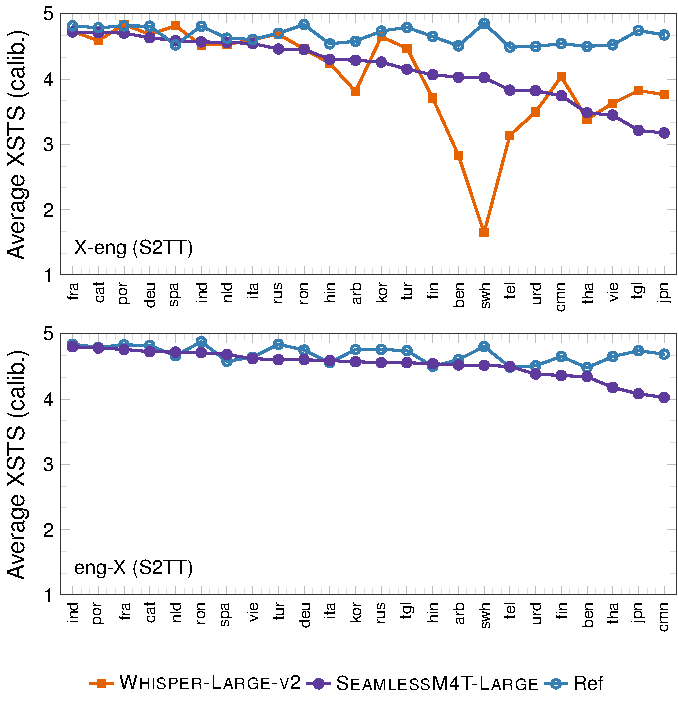
\includegraphics[width=0.8\textwidth]{figures/evaluation/xsts_calibrated_s2t.pdf}
\caption{\label{fig:XSTS_scores_cal_S2T} Language Direction level mean XSTS scores per direction for \st modality, after calibration. Bootstrapped 95\% CI is typically within $\sim\pm0.1$.}
\end{figure}

We present results for the \st task using the XSTS protocol (see Table \ref{table:evalsummary}). Figure \ref{fig:XSTS_scores_cal_S2T} shows calibrated XSTS scores on the language level for all models and languages evaluated (for both \xeng and \engx), which are also enumerated in Table \ref{table:fullXSTSresultsst} and summarized in Table \ref{tab:XSTShighlevelsummaryst}. For \xeng language directions, \mfourtlg quality was above an XSTS score of 3\footnote{The instructions surrounding an XSTS score of 3 are: ``The two sentences are mostly equivalent, but some unimportant details can differ.  There cannot be any significant conflicts in intent or meaning between the sentences, no matter how long the sentences are.''} for all \evallangs{} evaluated language directions. For \engx language directions, \mfourtlg was above an XSTS score of 4\footnote{The instructions for an XSTS score of 4 are: ``The two sentences are paraphrases of each other. Their meanings are near-equivalent,  with no major differences or information missing. There can only be minor differences in meaning due to differences in expression (e.g., formality level, style, emphasis, potential implication, idioms, common metaphors).''} for all \evallangs{} evaluated language directions.

Notably, in the \xeng direction, we see that \mfourtlg improves translation quality considerably over the \whisperlarge baseline for Swahili (an XSTS improvement of 2.38), Bengali (an XSTS improvement of 1.19), Telugu (an XSTS improvement of 0.69, and Modern Standard Arabic (an XSTS improvement of 0.47). \mfourtlg has significant improvements in language quality over \whisperlarge for 10 out of the \evallangs{} languages evaluated \xeng with regressions in 10, but only 2 languages, Japanese and Tagalog, have regressions of more than 0.5 XSTS.

When averaging over language directions, \mfourtlg demonstrates superior performance on both average XSTS score and percentage of sentences above XSTS thresholds of 3 and 4 compared to the \whisperlarge's baseline on \xeng (see Table \ref{tab:XSTShighlevelsummaryst}).

We also note generally higher performance in the \engx direction compared to the \xeng direction. From the automatic results in section \ref{subsec:multitaskingxtresults}, we observed that the higher performance in one direction or the other varies depending on the task (\st, \sst, or \mt). For \st, in terms of \spbleu and \blaser (see Table \ref{tbl:modeling:spbleu}), even when averaging over a larger set of languages, superior performance in \engx compared to \xeng holds. We offer a few possible explanations for this phenomenon. For example, speech encoding may be a more complicated task than speech or text decoding. If this is the case, better performance in English speech encoding could contribute to higher performance in the \engx direction. Data-wise, a plausible explanation could be a difference in audio quality of \fleurs recordings for different languages (e.g., English source sentence audio quality may have been higher, inflating the \engx scores), though evidence for this is only anecdotal. %

\paragraph{XSTS results for \sst task}

\begin{figure}
\centering
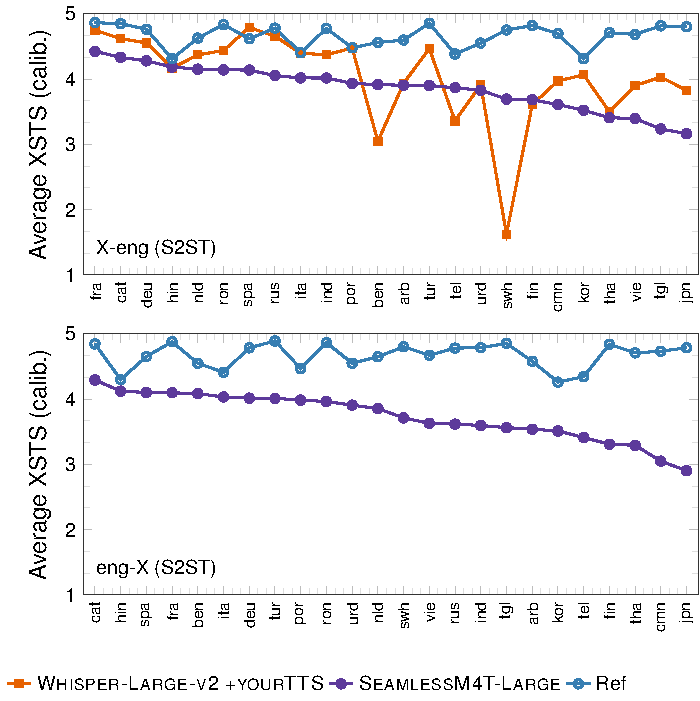
\includegraphics[width=0.8\textwidth]{figures/evaluation/xsts_calibrated_s2st.pdf}
\caption{\label{fig:XSTS_scores_cal_S2ST} Language Direction level mean XSTS scores per direction for \sst modality, after calibration. Bootstrapped 95\% CI is typically within $\sim\pm0.1$.}
\end{figure}

\begin{table}
\begin{tabular}{rrccc}
\toprule
{\bf Direction} & {\bf System} & {\bf Avg. XSTS (\sst)} & {\bf \% 3+} & {\bf \% 4+} \\
\midrule
\engx & Human reference & 4.67 & 95.38 & 79.45 \\
 & \mfourtlg & 3.73 & 58.10 & 36.90 \\
\midrule
 & Human reference & 4.66 & 95.20 & 78.89 \\
\xeng & \whisperlarge+\yourtts & {\bf 4.04} & {\bf 71.52} & {\bf 56.18} \\
 & \mfourtlg & 3.87 & 60.61 & 46.05 \\
\bottomrule
\end{tabular}
\caption{For \sst task: overall average XSTS human evaluation results into and out of English, over all \evallangs{} evaluated languages.  Results were computed for each language direction (see Table \ref{table:fullXSTSresultssst} for full language-level results).  \%3+ and  \%4+ refer to the percent of a language's evaluated sentences with median scores equal to or greater than 3 and 4 respectively.  Avg number of items is identical to those presented in Table \ref{tab:XSTShighlevelsummaryst}.}
\label{tab:XSTShighlevelsummarysst}
\end{table}


\begin{table}
\centering
\begin{threeparttable}
\scriptsize
\begin{tabular}{ll|ccc|ccc|ccc|c}
\toprule
\textbf{Direction} & \textbf{Lang} & \multicolumn{3}{c}{\textbf{XSTS (calibrated)}} & \multicolumn{3}{c}{\textbf{\% XSTS 3+}} & \multicolumn{3}{c}{\textbf{\% XSTS 4+}} & \textbf{Items} \\
 &  & Seamls\tnote{1} & Wspr\tnote{2} & Hum\tnote{3} & Seamls & Wspr & Hum & Seamls & Wspr & Hum &  \\
\midrule
\engx & arb & 3.55 & -- & 4.59 & 51.5 & -- & 95.4 & 24.9 & -- & 74.6 & 410 \\
 & ben & 4.09 & -- & 4.56 & 80.4 & -- & 96.8 & 41.0 & -- & 67.9 & 629 \\
 & cat & 4.3 & -- & 4.85 & 77.7 & -- & 98.3 & 64.3 & -- & 90.9 & 638 \\
 & cmn & 3.06 & -- & 4.74 & 31.4 & -- & 98.3 & 7.7 & -- & 72.2 & 636 \\
 & deu & 4.02 & -- & 4.79 & 63.4 & -- & 97.9 & 29.4 & -- & 72.4 & 612 \\
 & fin & 3.32 & -- & 4.84 & 32.3 & -- & 95.4 & 16.0 & -- & 85.9 & 632 \\
 & fra & 4.1 & -- & 4.88 & 64.5 & -- & 98.5 & 44.2 & -- & 87.2 & 538 \\
 & hin & 4.13 & -- & 4.3 & 94.6 & -- & 98.7 & 83.0 & -- & 95.1 & 388 \\
 & ind & 3.6 & -- & 4.8 & 58.1 & -- & 98.2 & 35.5 & -- & 93.0 & 544 \\
 & ita & 4.04 & -- & 4.42 & 86.8 & -- & 100.0 & 75.8 & -- & 96.1 & 612 \\
 & jpn & 2.91 & -- & 4.79 & 18.5 & -- & 91.6 & 11.1 & -- & 80.5 & 514 \\
 & kor & 3.52 & -- & 4.27 & 40.2 & -- & 77.0 & 13.8 & -- & 39.9 & 356 \\
 & nld & 3.86 & -- & 4.65 & 52.2 & -- & 90.4 & 32.8 & -- & 58.8 & 335 \\
 & por & 3.99 & -- & 4.47 & 81.6 & -- & 99.1 & 70.7 & -- & 94.6 & 632 \\
 & ron & 3.97 & -- & 4.87 & 63.3 & -- & 97.1 & 42.2 & -- & 89.2 & 619 \\
 & rus & 3.62 & -- & 4.78 & 40.4 & -- & 93.6 & 29.5 & -- & 75.0 & 597 \\
 & spa & 4.11 & -- & 4.66 & 64.2 & -- & 96.5 & 47.2 & -- & 63.7 & 623 \\
 & swh & 3.72 & -- & 4.8 & 45.1 & -- & 91.6 & 34.8 & -- & 84.5 & 466 \\
 & tel & 3.42 & -- & 4.35 & 60.0 & -- & 91.9 & 24.0 & -- & 61.8 & 442 \\
 & tha & 3.3 & -- & 4.72 & 46.7 & -- & 95.6 & 21.5 & -- & 86.2 & 643 \\
 & tur & 4.02 & -- & 4.89 & 65.4 & -- & 98.8 & 32.9 & -- & 87.8 & 566 \\
 & urd & 3.91 & -- & 4.56 & 71.7 & -- & 94.3 & 40.3 & -- & 71.0 & 283 \\
 & vie & 3.64 & -- & 4.68 & 64.5 & -- & 98.4 & 43.2 & -- & 91.0 & 611 \\
 \midrule
\xeng & arb & 3.91 & 3.94 & 4.61 & 62.2 & 68.0 & 96.1 & 48.5 & 50.7 & 75.6 & 410 \\
 & ben & 3.92 & 3.05 & 4.57 & 68.0 & 43.7 & 96.5 & 38.2 & 15.1 & 69.6 & 629 \\
 & cat & 4.34 & 4.63 & 4.86 & 77.7 & 88.7 & 98.4 & 68.8 & 82.4 & 91.4 & 638 \\
 & cmn & 3.62 & 3.98 & 4.7 & 51.1 & 67.6 & 97.0 & 26.7 & 36.6 & 68.6 & 636 \\
 & deu & 4.29 & 4.56 & 4.77 & 69.9 & 85.0 & 95.6 & 49.3 & 60.0 & 72.5 & 612 \\
 & fin & 3.69 & 3.62 & 4.82 & 44.3 & 44.9 & 94.6 & 33.1 & 29.1 & 84.7 & 632 \\
 & fra & 4.43 & 4.75 & 4.87 & 75.1 & 92.2 & 98.3 & 64.5 & 80.9 & 85.7 & 538 \\
 & hin & 4.19 & 4.18 & 4.32 & 95.6 & 95.6 & 99.0 & 88.4 & 89.7 & 95.4 & 388 \\
 & ind & 4.02 & 4.38 & 4.78 & 67.3 & 84.2 & 97.6 & 57.2 & 76.1 & 92.5 & 544 \\
 & ita & 4.02 & 4.4 & 4.41 & 82.0 & 98.4 & 99.3 & 76.3 & 96.4 & 96.1 & 612 \\
 & jpn & 3.17 & 3.84 & 4.81 & 26.7 & 51.0 & 92.8 & 20.2 & 39.9 & 81.3 & 514 \\
 & kor & 3.53 & 4.07 & 4.32 & 40.4 & 66.0 & 82.0 & 18.5 & 37.1 & 40.7 & 356 \\
 & nld & 4.16 & 4.38 & 4.63 & 58.5 & 71.9 & 89.6 & 49.9 & 54.6 & 55.8 & 335 \\
 & por & 3.94 & 4.48 & 4.49 & 74.7 & 98.7 & 99.4 & 70.1 & 96.2 & 95.9 & 632 \\
 & ron & 4.15 & 4.44 & 4.84 & 67.9 & 81.1 & 96.4 & 52.0 & 65.9 & 86.9 & 619 \\
 & rus & 4.06 & 4.66 & 4.78 & 55.4 & 82.6 & 92.5 & 46.1 & 74.2 & 76.2 & 597 \\
 & spa & 4.15 & 4.79 & 4.62 & 65.2 & 93.4 & 95.7 & 52.5 & 83.6 & 61.2 & 623 \\
 & swh & 3.7 & 1.63 & 4.76 & 41.2 & 1.3 & 89.7 & 32.6 & 0.9 & 80.0 & 466 \\
 & tel & 3.87 & 3.37 & 4.39 & 72.6 & 58.1 & 94.8 & 44.3 & 30.1 & 62.9 & 442 \\
 & tha & 3.42 & 3.51 & 4.72 & 48.8 & 56.0 & 95.6 & 31.9 & 33.4 & 86.6 & 643 \\
 & tur & 3.91 & 4.47 & 4.86 & 57.8 & 81.3 & 97.3 & 37.1 & 62.4 & 85.5 & 566 \\
 & urd & 3.84 & 3.92 & 4.56 & 66.8 & 72.4 & 92.6 & 40.6 & 48.4 & 72.1 & 283 \\
 & vie & 3.4 & 3.91 & 4.69 & 53.7 & 73.0 & 98.4 & 37.6 & 57.8 & 92.5 & 611 \\
\bottomrule
\end{tabular}
\begin{tablenotes}
\item[1] \mfourtlg
\item[2] \whisperlarge
\item[3] Human reference
\end{tablenotes}
\end{threeparttable}
\caption{\label{table:fullXSTSresultssst} Full calibrated XSTS \sst results; bootstrapped 95\% CI widths are $\sim\pm 0.1$ on average.  \%3+ and \%4+ refer to the percent of a language’s evaluated sentences with median (uncalibrated) XSTS scores equal to or greater than 3 and 4 respectively.}
\end{table}


Figure \ref{fig:XSTS_scores_cal_S2ST} shows aggregate, language-level XSTS scores for the \sst task, which are also presented in Table \ref{table:fullXSTSresultssst} and summarized in Table \ref{tab:XSTShighlevelsummarysst}. In the \xeng direction, where a \whisperlarge+\yourtts baseline has been evaluated, we see that XSTS scores for \mfourtlg tend to lag behind the baseline, with the notable exceptions of Bengali, Telugu, and Swahili (where \mfourtlg scores significantly higher than the \whisperlarge+\yourtts baseline). In aggregate, \mfourtlg still performs reasonably well, with the majority of language directions scoring at or above an XSTS score of 3.

XSTS \sst performance of \mfourtlg is in sharp contrast to two results: one is \st performance, where \mfourtlg is roughly on par with \whisperlarge and far surpasses performance in a few tested languages (most notably Swahili) in both XSTS and automated metrics (\blaser and \bleu), the other is \sst performance in terms automated metrics (\blaser and \asrbleu), where \mfourtlg consistently outperforms \whisperlarge+\yourtts baseline in the \xeng direction.

When moving from \st to the \sst task, language-level XSTS scores decreased by an average of 0.29 points for the \mfourtlg model but remained virtually unchanged (a decrease of only 0.01 points) for the \whisperlarge+\yourtts baseline.

Additionally, XSTS annotators report ``audio issues'' for \mfourtlg generations much more frequently, by almost an order of magnitude, than \whisperlarge+\yourtts generations (on \xeng direction, 206 \mfourtlg \sst generations were reported as having ``audio issues'' by at least one annotator, compared to only 22 \whisperlarge+\yourtts \sst generations and 13 human reference items; in \texttt{fra} (\xeng) for example, more than 10\% of \mfourtlg items were marked as having audio issues by at least one annotator). Excluding items marked as having audio issues by at least one annotator does not increase \mfourtlg XSTS scores appreciably (only 3 languages \xeng have XSTS score increases of slightly more than 0.1 when audio issue items are removed, and the rest have XSTS increases of less than 0.04), but high incidence of reported ``audio issues'' may be a symptom of a  problem that does correspond to the observed performance decrease of \mfourtlg on the \sst task in XSTS.

\paragraph{Truncation and omission in \sst output}

\begin{figure}
\centering
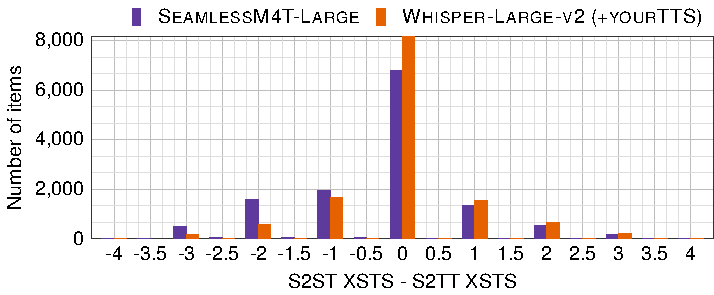
\includegraphics[width=0.9\textwidth]{figures/evaluation/xsts_s2st_s2tt_deltas_item_level.pdf}
\caption{\label{fig:xsts_delta_histogram} XSTS score differences between \sst and \st generations at the item level. A higher proportion of \mfourtlg \sst generations received XSTS scores that are 2 or more points behind the \st generation compared to \whisperlarge(+\yourtts).}

\end{figure}

Figure \ref{fig:xsts_delta_histogram} shows a histogram of performance deltas between \sst and \st generations for both \mfourtlg and \whisperlarge(+\yourtts). We see that \mfourtlg has a higher proportion of items with \sst generations 2 or more XSTS points behind the \st generation.


These observations motivated a small-scale inspection of 50 randomly sampled items (25 generations from \mfourtlg and 25 generations from \whisperlarge+\yourtts) where the median XSTS score was 5 for the \st generation but less than 4 for the \sst generation. We discovered that half of the sampled items in the \whisperlarge+\yourtts generations had poor \st translation quality but still received high marks. In the \mfourtlg sample, we similarly found that about half of the sampled items had a poor \st translation quality but still received a high score for the \st translation. Note that such a high proportion of XSTS scores not reflecting underlying performance in this inspection is not particularly surprising; we are conditioning on a score mismatch between modalities, and one common reason for a score mismatch is an errant score. However, in addition to this, half of the samples had the end of the \st translation truncated in the generated \sst audio (which did not occur in the sample of \whisperlarge+\yourtts generations). Truncations may have had a small impact on automated measures like \asrbleu but a large impact on the underlying meaning, and this may be reflected in the XSTS scores. The impact of a truncation or omission likely varies depending on which words are truncated or omitted; the distribution of performance deltas shown in Figure \ref{fig:xsts_delta_histogram} seem consistent with a mix of both minor and major impacts to underlying meaning.

If truncations are the predominant reason behind the drop in XSTS scores for \mfourtlg in the \sst task, one possible aggravating factor may be recency bias: due to truncations being the most recent effect an annotator observes, their perceived importance on translation quality may be higher. This may be especially true in the \sst task, where simultaneous comparison of source and target is difficult due to both being in the speech modality; if cognitive load is too high this may reduce an annotator's ability to holistically reflect on the quality of the entire translation and may further exacerbate the effect of recency bias.


\paragraph{\st and \sst performance as a function of source audio duration}
\begin{figure}
\centering
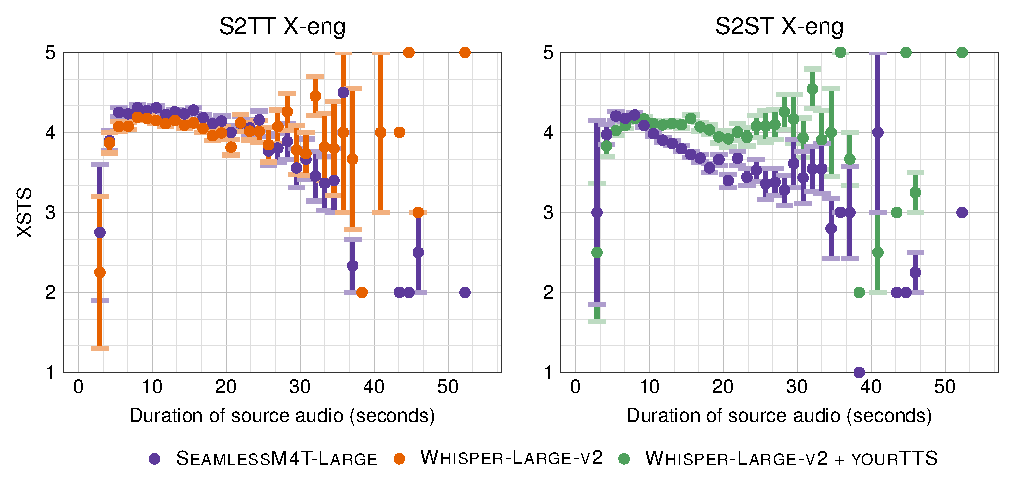
\includegraphics[width=0.8\textwidth]{figures/evaluation/performance_vs_source_audio_duration_v2}
\caption{\label{fig:perf_vs_src_duration} \st and \sst item-level XSTS scores as a function of the duration of the source speech audio file. Error-bars are standard errors around the mean in each source duration bucket.}
\end{figure}


Figure \ref{fig:perf_vs_src_duration} shows a breakdown of XSTS score by duration of source audio for both \st and \sst tasks for \mfourtlg and \whisperlarge(+\yourtts). We see that for the \st task, \mfourtlg provides superior performance over \whisperlarge on average item-level XSTS for most source audio durations, though performance for both models tends to decline for as a function of source audio duration for audios longer than $\sim$10 seconds. On the \sst task, \mfourtlg provides superior performance over \whisperlarge+\yourtts for shorter audio durations ($\lesssim$ 8 s) but \mfourtlg performance falls off rapidly for longer source audio durations compared to \whisperlarge+\yourtts performance which remains relatively stable for a broader range of source audio durations. This is consistent with the hypothesis that truncations and omissions are primarily responsible for the XSTS performance gap between \mfourtlg and \whisperlarge+\yourtts despite clear superiority of \mfourtlg on automated metrics, as longer source audios may more likely to suffer from truncations and omissions in the target audio.

 




\paragraph{MOS Results}

\begin{figure}
\centering
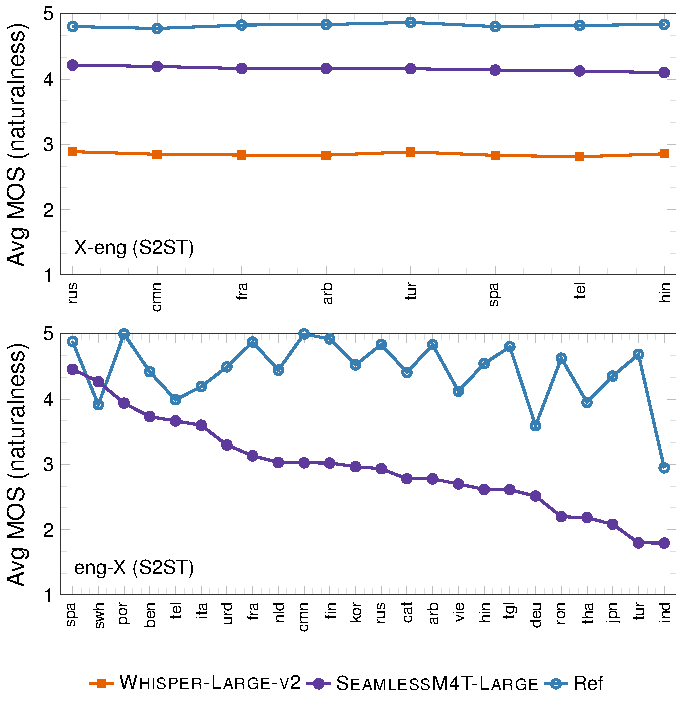
\includegraphics[width=0.8\textwidth]{figures/evaluation/mos_naturalness_s2st.pdf}
\caption{\label{fig:MOS_naturalness} Language Direction level mean MOS (naturalness) scores per direction for \sst modality, after calibration. Bootstrapped 95\% CI widths are $\sim\pm 0.1$ on average.}
\end{figure}


Figure \ref{fig:MOS_naturalness} presents language-level results for both \engx and \xeng translation directions on the ``naturalness'' aspect of the MOS protocol. 

In the \xeng direction, \mfourtlg shows superior performance in the naturalness MOS aspect compared to \whisperlarge+\yourtts. The consistency of MOS score across input languages in the \xeng direction is likely due to two major factors. One, the input speech is unlikely to affect output speech quality with respect to any of the aspects measured by MOS. Two, since MOS requires only a review of the target audio, the items from each input language were evaluated by the same set of 31 annotators. With each annotator scoring a similar fraction of items for each input language, the annotator bias effects are similar across source languages.

In the \engx direction, \texttt{spa} and \texttt{swh} generations received MOS naturalness scores above 4, and 11 directions received naturalness scores above 3. Additionally, we also measured ``Clarity of Speech'' and ``Sound Quality'' MOS aspects. We find that for languages where both \whisperlarge+\yourtts and \mfourtlg were measured (all \xeng), \mfourtlg averaged 0.67 points higher in sound quality and 0.79 points higher in clarity of speech over \whisperlarge+\yourtts (\mfourtlg surpassed the human reference in the ``clarity of speech'' and ``sound quality'' aspects for all 8 \xeng languages measured). In the \engx direction, for the ``clarity of speech'' aspect, 20 languages scored above a 3 for \mfourtlg, with 4 languages scoring above a 4; for the ``sound quality'' aspect, all languages scored above a 3, with 13 languages scoring above a 4.


\paragraph{Correlations between \asrbleu, \bleu and XSTS}
\begin{table}
\centering
\begin{tabular}{lll|cc}
\toprule
\textbf{Modality} & \textbf{Direction} & \textbf{Metric} & \textbf{Pearson} & \textbf{Spearman} \\
\toprule
\st & \engx & \blaser & \textbf{0.750} & \textbf{0.505} \\
 &  & \bleu & 0.053 & 0.355 \\

& \xeng & \blaser & \textbf{0.923} & \textbf{0.871} \\
&  & \bleu & 0.822 & 0.776 \\
& All & \blaser & \textbf{0.913} & \textbf{0.827} \\
&  & \bleu & 0.626 & 0.625 \\
\midrule
\sst & \engx & \blaser & \textbf{0.727} & \textbf{0.675} \\
 &  & \asrbleu & 0.154 & 0.292 \\

& \xeng & \blaser & \textbf{0.854} & \textbf{0.756} \\
&  & \asrbleu & 0.692 & 0.651 \\

& All & \blaser & \textbf{0.810} & \textbf{0.736} \\
&  & \asrbleu & 0.514 & 0.561 \\
\bottomrule
\end{tabular}
\caption{\label{tab:automated_metric_xsts_correlations} Comparison of language-level correlations between automated metrics and XSTS. \blaser provides superior correlations with human metrics in all directions, and modalities, with a particular improvement in correlations for \engx directions. These results hold for both Pearson and Spearman correlation coefficients.}
\end{table}


In Table \ref{tab:automated_metric_xsts_correlations} and visualized in Figure \ref{fig:auto_metric_corrs}, we compare the strength of correlations between automated metrics (\asrbleu for \sst and \bleu for \st) and XSTS at the language level. \asrbleu and \bleu are computed using corpus scores, and language level \blaser scores are computed by averaging sentence-level (supervised) \blaser scores over the evaluation set. All automated metrics are calculated using only the items sent for human evaluation with XSTS in order to make consistent comparisons, however \asrbleu and \blaser scores on the language level differed only slightly from those used to generate Tables \ref{tbl:modeling:cascaded:s2st} and \ref{tbl:modeling:cascaded:x2t}.

We find that, both with Spearman and Pearson correlation coefficients, \blaser has a superior correlation with XSTS over \asrbleu (for \sst task) and \bleu (for \st task), and \blaser correlates much better with XSTS in the \engx direction in particular. 


\begin{figure}
\centering
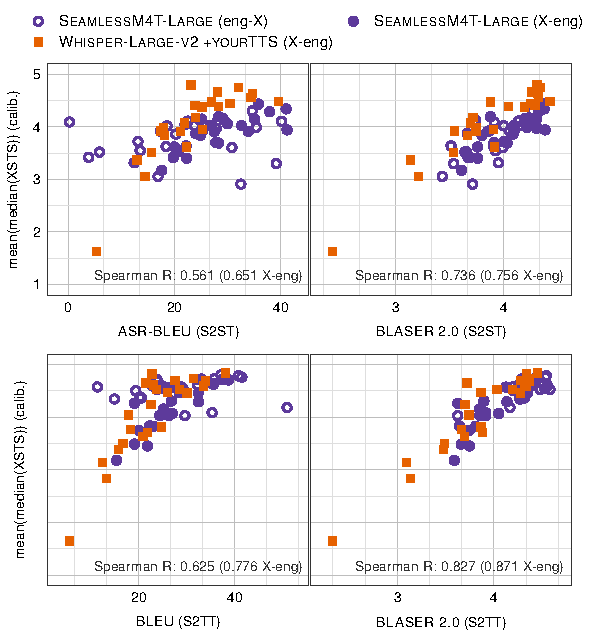
\includegraphics[width=0.8\textwidth]{figures/evaluation/automatic_metric_corrs_v2.pdf}
\caption{\label{fig:auto_metric_corrs} Correlations between XSTS and \asrbleu and \blaser for \sst task and between XSTS and \bleu and \blaser for \st task. \blaser offers superior correlation with XSTS, most notably for \engx directions where \asrbleu and \bleu correlations are much weaker than for \xeng directions.}
\end{figure}





\subsubsection{Limitations}

\textbf{Test set limitations} The \fleurs \citep{fleurs2022arxiv} test set is limited in that the different language pairs contain slightly different sets of sentences. Due to the limitations in both the dataset (which contains a maximum of 3 speakers) and timing and cost considerations on the human evaluation front (we evaluated a maximum of two speakers per sentence), we have a lack of diversity in our speaker set per language, which may introduce bias relative to a test set with a larger number of speakers.


\noindent \textbf{Limited sample size of human annotators per language} We only have a maximum of 5 (but typically 3) annotator evaluations per sentence for each language in our XSTS evaluations. Relatively small samples of annotators mean annotator bias is important to consider. We try to mitigate this by (1) using the median score per sentence for each language to be robust to outliers, (2) using bootstrap re-sampling of annotator scores to estimate language score uncertainty due to finite annotators, and (3) approximate and correct annotator bias with a cross-lingual calibration set. For MOS, several language directions only have a single annotator per item, with no calibration set—this exacerbates issues related to annotator bias.


\noindent \textbf{Challenges of implementing reliable human measures of performance} Obtaining human measures of translation performance offers several advantages over automated metrics (e.g. while \bleu-like metrics are trivial to ``game'', humans are not as easily fooled, and humans are better judges of target translations of high quality but for which word content differs from available reference translations), but human measures of translation quality suffer from their own limitations that are not shared by automated metrics. XSTS was designed to mitigate some of these limitations (annotator bias and variance) but, e.g., recency bias and other human biases may still persist. We continue to develop additional recommendations and clarifications, improve annotator trainings and reduce cognitive load, but obtaining reliable human measures of translation quality continues to be an active area of research and development.

\subsection{Automatic Robustness Evaluation}
\label{subsec:appendix:robustness}

We evaluated model robustness against non-linguistic perturbations in the real-world speech inputs, including background noises and speaker variations. As reported in several other sections, we compare our model to \whisperlarge.%

\subsubsection{Robustness Against Background Noises}

\begin{figure}[t]
    \centering
    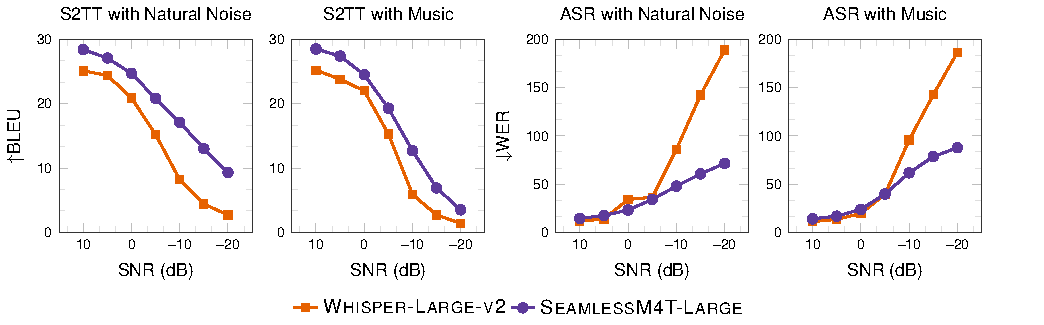
\includegraphics[width=1.1\linewidth]{figures/evaluation/noise_robustness_row.pdf}
    \caption{\textbf{Evaluation results of model robustness against background noises.} We report average test \bleu and test \wer over 4 languages (3 language families) for \xeng~\st and ASR on \fleurs with low-to-high input noise level (high-to-low SNR). Simulated noises are sampled from MUSAN~\citep{snyder2015musan} on the ``noise'' and ``music'' categories.}
    \label{fig:robustness_noise}
\end{figure}

\paragraph{Related work} The analysis of speech model robustness across different background noise levels has been conducted in prior work~\citep{wang2022wav2vec,zhu2022noise,whisper} on simulated noisy audios. However, existing simulation-based evaluations are either limited by the noise types (e.g., simple white noise), task coverage (e.g., ASR only), language coverage (e.g., English only), or the replicability of benchmark data. This calls for an open, versatile benchmark to overcome these limitations.


\paragraph{Experimental framework} We build a replicable noise-robustness evaluation benchmark based on \fleurs ("noisy \fleurs''), which covers 102 languages, 2 speech tasks (\st and ASR), and various noise types (natural noises and music). To create simulated noisy audios, we sampled audio clips from MUSAN~\citep{snyder2015musan} on the ``noise'' and ``music'' categories, and mixed them with the original \fleurs speech audios under different signal-to-noise ratio (SNR): 10, 5, 0, -5, -10, -15 and -20. We compare models by \bleu-SNR curves (for \st) or \wer-SNR curves (for ASR), which illustrate the degree of model performance degradation when the noise level of speech inputs increases (i.e., when SNR decreases). Both \mfourtlg and \whisperlarge achieve high performance mostly in high-resource languages, where stress tests in the noisy speech setup are more necessary and informative. For low-resource languages, the clean speech setup is already challenging, let alone the noisy one. We hence focus on 4 high-resource languages (French, Spanish, Modern Standard Arabic, and Russian) from 3 different language families for our noise-robustness analysis on \mfourtlg and \whisperlarge.

\paragraph{Results} Figure~\ref{fig:robustness_noise} shows the average test \bleu and test \wer over the 4 languages for \xeng{} \st and \asr on \fleurs with low-to-high input noise level (high-to-low SNR). We see that both \bleu-SNR curves for \mfourtlg are consistently above those for \whisperlarge. Similarly, \mfourtlg's \wer-SNR curves are consistently below \whisperlarge's ones. These suggest the superior robustness of \mfourtlg in noisy speaking environments. \mfourtlg outperforms \whisperlarge by an average of 33.3\% and 42.2\% over various noise types and noise levels for \xeng{} \st and \asr, respectively.



\subsubsection{Robustness Against Speaker Variations}
\label{subsec:robustnessspeakervariation}

\paragraph{Related work} \asr and \st systems are expected to minimize the effects of speaker variations that are irrelevant to the input content of interest. Fairness of \asr systems to different speaker subgroups (by race, gender, country, etc.) has been studied in prior work~\citep{liu2022towards,dheram2022toward}, which requires the availability of accurate speaker demographics labels~\citep{hazirbas2021casual,porgali2023casual} for speaker grouping and group-wise scoring. However, these labels are rare in existing \asr benchmarks, limiting the applications of such analysis. To overcome label scarcity, \cite{wang-etal-2020-covost} proposed a set of label-free metrics that do not rely on speaker grouping for analyzing the effects of speaker variations.

\paragraph{Experimental setup} We follow~\cite{wang-etal-2020-covost} to evaluate model robustness against speaker variations by calculating average by-group mean score and by-group coefficient of variation of an utterance-level quality metric. Instead of using \bleu as the quality metric, we used chrF, which has better stability at the utterance level. The calculation of both robustness metrics does not require explicit speaker subgroup labels. We grouped evaluation samples and corresponding utterance-level chrF scores by content (transcript), and then calculated the average by-group mean score $\textrm{chrF}_{MS}$ and average by-group coefficient of variation $\textrm{CoefVar}_{MS}$ defined as follows:
\begin{align*}
    \textrm{chrF}_{MS}&=\frac{1}{|G|}\sum_{g\in G}\textrm{Mean}(g) \\
    \textrm{CoefVar}_{MS}&=\frac{1}{|G'|}\sum_{g\in G'}\frac{\textrm{StandardDeviation}(g)}{\textrm{Mean}(g)}
\end{align*}
where $G$ is the set of sentence-level chrF scores grouped by content (transcript) and
$G' = \{g | g\in G, |g|>1, \textrm{Mean}(g) > 0 \}$.
The two metrics are complementary: $\textrm{chrF}_{MS}$ provides a normalized quality metric that, unlike conventional corpus-level metrics, takes speaker variations into consideration, while $\textrm{CoefVar}_{MS}$ provides a standardized measure of quality variance under speaker variations. 
For robustness analysis of \mfourtlg and \whisperlarge, we conducted an out-of-domain evaluation on \fleurs on all its languages that have at least 40 content groups in the test sets.

\begin{table}[htb]
    \centering
    \small
    \begin{tabular}{lccccc}
        \toprule
        \multirow{1}{*}{\bf Languages} & \multirow{1}{*}{\bf Average \#} &  \multicolumn{2}{c}{\bf \whisperlarge} & \multicolumn{2}{c}{\bf \mfourtlg} \\
        \cmidrule(lr){3-4} \cmidrule(lr){5-6}
        ($\ge$ 40 content groups) & cont. groups & chrF$_{MS}$$\uparrow$ & CoefVar$_{MS}$$\downarrow$ & chrF$_{MS}$$\uparrow$ & CoefVar$_{MS}$$\downarrow$ \\
        \midrule[\heavyrulewidth]
        \xeng~\st for 77 langs & 278 & 40.8 & 13.7 & \textbf{45.3} & \textbf{9.1} \\
        \asr for 78 langs & 280 & 58.7 & 17.0 & \textbf{72.5} & \textbf{6.4} \\
        \bottomrule
    \end{tabular}
\caption{\textbf{Evaluation results of model robustness against speaker variations.} We report average by-group mean chrF (chrF$_{MS}$) and average by-group coefficient of variation on chrF (CoefVar$_{MS}$) on \fleurs \xeng \st and ASR test sets.}
\label{tbl:robustness-speaker-variation}
\end{table}

\paragraph{Results} Table~\ref{tbl:robustness-speaker-variation} shows the $\textrm{chrF}_{MS}$ and $\textrm{CoefVar}_{MS}$ scores of \mfourtlg and \whisperlarge on \fleurs~\xeng~\st and \asr test sets. We see that \mfourtlg outperforms \whisperlarge on $\textrm{CoefVar}_{MS}$ by an average of 49.4\% over the 2 tasks. Moreover, \mfourtlg outperforms \whisperlarge on chrF$_{MS}$ by an average of 18.3\%. These suggest the superior robustness of \mfourtlg when it comes to speaker variations.








